\documentclass{standalone}
\usepackage{tikz}

\begin{document}

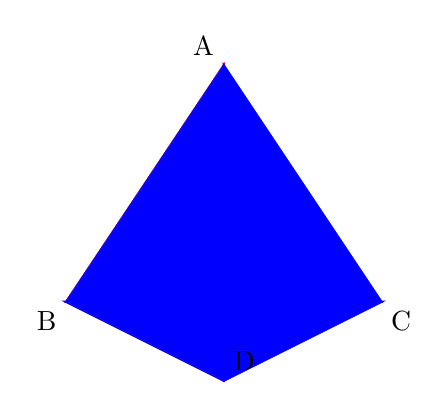
\begin{tikzpicture}[scale=2]
    % Define points
    \coordinate (A) at (0, 1);
    \coordinate (B) at (-1, -0.5);
    \coordinate (C) at (1, -0.5);
    \coordinate (D) at (0, -1);

    % Draw edges
    \draw[thick, red] (A) -- (B) -- (D) -- cycle; % Bottom face (red)
    \draw[thick, blue] (A) -- (C) -- (D) -- cycle; % Top face (blue)
    \draw[thick, blue] (A) -- (B) -- (C) -- cycle; % Side face (blue)
    \draw[thick, blue] (B) -- (C) -- (D) -- cycle; % Side face (blue)

    % Fill faces with colors
    \fill[red] (A) -- (B) -- (D) -- cycle;
    \fill[blue] (A) -- (C) -- (D) -- cycle;
    \fill[blue] (A) -- (B) -- (C) -- cycle;
    \fill[blue] (B) -- (C) -- (D) -- cycle;

    % Add labels (optional)
    \node at (A) [above left] {A};
    \node at (B) [below left] {B};
    \node at (C) [below right] {C};
    \node at (D) [above right] {D};

\end{tikzpicture}

\end{document}